\section{Aritmetica di macchina}

Cerchiamo ora di estendere l'aritmetica tra numeri reali ad un'aritmetica per i numeri di macchina. Il primo tentativo è quello di usare semplicemente le solite operazioni definite tra numeri reali, tuttavia non è detto che il risultato di un'operazione tra numeri di macchina sia ancora un numero di macchina.

\begin{example}
    Consideriamo il sistema $\MSet{10, 3, -5, 5}$ e i due numeri di macchina \[
        a \deq 123 = 10^3 (0.123)_{10}, \qquad b \deq 0.456 = 10^0 (0.456).
    \] Si ha che $a,\ b \in \MSet{10, 3, -5, 5}$, tuttavia $a + b = 123.456 = 10^3 (0.123456)_{10}$ non è un numero di macchina poiché è rappresentato con $t = 6$ cifre di precisione.
\end{example}

Dobbiamo quindi definire delle nuove operazioni che siano \emph{interne} all'insieme dei numeri di macchina.

\begin{definition}
    [Aritmetica di macchina] Si definiscono quattro operazioni \[
        \oplus,\ \otimes,\ \ominus,\ \oslash : \MSet \times \MSet \to \MSet
    \] tali che per ogni coppia di numeri di macchina $a, b \in \MSet$ ($b \neq 0$ nel caso di $\oslash$) si ha che \begin{align*}
        &a \oplus b \deq \fl{a + b} &&a \ominus b \deq \fl{a - b}\\
        &a \otimes b \deq \fl{ab}   &&a \oslash b \deq \fl{\nicefrac{a}{b}}
    \end{align*}
\end{definition}

Siamo ora interessati a studiare \emph{quanto errore} commettiamo nel considerare i numeri di macchina invece dei numeri reali non approssimati.

\begin{definition}
    [Errore locale]
    Sia $\ast$ un'operazione tra numeri qualsiasi e sia $\circledast$ la corrispondente operazione su numeri di macchina. Dati $x, y \in \FF$ si dice \strong{errore locale} dell'operazione la quantità \[
        \eps \deq \frac{(x \circledast y) - (x \ast y)}{x \ast y}.
    \]
\end{definition}

Osserviamo che ogni operazione di macchina può essere scritta in termini della sua corrispondente operazione base e dell'errore locale: in effetti \[
    x \circledast y = (x \ast y)(1 + \eps).
\]

\begin{example}[Errore nel calcolo della somma]

Cerchiamo ora di calcolare l'errore totale commesso nell'approssimazione di un'operazione tra numeri reali (definiremo più avanti precisamente il concetto di errore totale). Prendiamo $a, b \in \R$ che approssimati non vadano in overflow (o underflow) e cerchiamo di calcolare $a + b$ in termini di numeri di macchina.

Siccome i numeri $a,\ b$ non sono necessariamente già numeri di macchina, l'unico modo per svolgere il calcolo è calcolare la quantità \[
    \tilde a \oplus \tilde b = (\tilde a + \tilde b)(1 + \eps).
\] Siccome sappiamo che, se $\eps_a,\ \eps_b$ sono gli errori di rappresentazione rispettivamente di $a$ e $b$ \begin{align*}
    &\tilde a = a(1 + \eps_a), \quad \tilde b = b(1 + \eps_b)
\end{align*} otteniamo che \begin{align*}
    \tilde a \oplus \tilde b 
        &= (a(1 + \eps_a) + b(1 + \eps_b))(1 + \eps)\\
        &= a(1 + \eps_a)(1 + \eps) + b(1 + \eps_b)(1 + \eps).
    \intertext{Nello svolgere il prossimo passaggio trascureremo gli addendi in cui compare il prodotto di due errori: effettueremo quindi un'\strong{analisi al primo ordine}, indicata dal simbolo $\doteq$.}
        &\doteq a + b + a\eps_a + b\eps_b + (a+b)\eps.
\end{align*}

L'errore complessivo che commettiamo è quindi dato dalla differenza tra il risultato ottenuto ($\tilde a \oplus \tilde b)$ e il risultato non approssimato ($a + b$), dividendo per il risultato non approssimato in modo da ottenere un errore relativo: \begin{align*}
    \frac{(\tilde a \oplus \tilde b) - (a + b)}{a + b} 
    &\doteq \frac{a + b + a\eps_a + b\eps_b + (a+b)\eps - (a + b)}{a + b} \\
    &= \frac{a}{a+b}\eps_a + \frac{b}{a + b}\eps_b + \eps.
\end{align*}

Notiamo che questo errore può essere diviso in due parti diverse:
\begin{itemize}
    \item la parte data da $\frac{a}{a+b}\eps_a + \frac{b}{a+b}\eps_b$ non dipende dal tipo di operazione che sto cercando di svolgere, ma dal fatto che devo approssimare gli argomenti dell'operazione: lo chiameremo \strong{errore inerente};
    \item la parte data da $\eps$ dipende dalla sequenza di passi scelta per calcolare la somma: lo chiameremo perciò \strong{errore algoritmico}.    
\end{itemize}
\end{example}

\begin{example}[Errore di una funzione]
    \label{exmpl:func_error}
Consideriamo la funzione $f : \R \to \R$ definita da \[
    f(x) = x^2 - 1.
\]
Calcoliamo l'errore totale commesso nel calcolare $f(x)$ tramite operazioni di macchina.

Osserviamo che potenzialmente abbiamo più \emph{algoritmi} (intesi come sequenze di calcoli) per calcolare $f$: scegliamo ad esempio gli algoritmi di macchina $g_1$, $g_2$ definiti da \[
    g_1(\tilde x) \deq (\tilde x \otimes \tilde x) \ominus 1, \qquad g_2(\tilde x) \deq (\tilde x \ominus 1) \otimes (\tilde x \oplus 1).
\] 

L'algoritmo $g_1$ prescrive di calcolare innanzitutto $z \deq \tilde x \otimes \tilde x$ e dopo calcolare $z \ominus 1$. Se $\eps_1$ è l'errore locale dell'operazione $\otimes$ si ha che \[
    z = \tilde{x}^2 (1 + \eps_1);
\] chiamando $\eps_2$ l'errore locale dell'operazione $\ominus$ si ottiene \begin{equation*}
    g_1(\tilde x) = (z - 1)(1 + \eps_2).
\end{equation*}
A questo punto, ricordando che $\tilde x = x(1 + \eps_x)$ dove $\eps_x$ è l'errore di rappresentazione, si può esprimere $g_1(\tilde x)$ in termini di $x$ e dei vari errori. In effetti
\begin{align*}
        &(z - 1)(1 + \eps_2)\\
    = {}&\parens[\big]{\tilde{x}^2 (1 + \eps_1) - 1}(1 + \eps_2)\\
    = {}&\parens[\Big]{\parens[\big]{x(1+\eps_x)}^2(1 + \eps_1) - 1}(1 + \eps_2)\\
    = {}&\parens[\big]{x^2(1+\eps_x)^2(1 + \eps_1) - 1}(1 + \eps_2)\\
    \doteq {}&\parens[\big]{x^2(1+2\eps_x)(1 + \eps_1) - 1}(1 + \eps_2)\\
    \doteq {}&\parens[\big]{x^2(1+2\eps_x + \eps_1) - 1}(1 + \eps_2)\\
    = {}&x^2(1+2\eps_x + \eps_1)(1 + \eps_2) - (1 + \eps_2)\\
    \doteq {}&x^2(1 + 2\eps_x + \eps_1 + \eps_2) - (1 + \eps_2)\\
    = {}&x^2 -1 + 2x^2\eps_x + x^2\eps_1 + (x^2-1)\eps_2.
\end{align*}
L'errore totale commesso nell'approssimare il risultato della funzione $f(x)$ con la funzione di macchina $g_1(\tilde x)$ è dunque \begin{align*}
    \eps_{g_1} &\deq \frac{x^2 -1 + 2x^2\eps_x + x^2\eps_1 + (x^2-1)\eps_2 - (x^2-1)}{x^2 - 1}\\
    &= \frac{2x^2}{x^2 - 1}\eps_x + \frac{x^2}{x^2-1}\eps_1 + \eps_2.
\end{align*}

Ripetiamo il procedimento per l'algoritmo $g_2$: siano $\delta_1,\ \delta_2$ e $\delta_3$ i tre errori locali commessi; ovvero \begin{align*}
    z_1 &\deq \tilde{x} \ominus 1 = (\tilde x - 1)(1 + \delta_1)\\
    z_2 &\deq \tilde{x} \oplus 1 = (\tilde x + 1)(1 + \delta_2)\\
    g_2(\tilde x) &= z_1 \otimes z_2 = z_1z_2(1 + \delta_3).
\end{align*}
Si ha quindi \begin{align*}
    &z_1z_2(1+\delta_3)\\
    = {}&(\tilde x - 1)(1 + \delta_1)(\tilde x + 1)(1 + \delta_2)(1 + \delta_3)\\
    = {}&(\tilde{x}^2 - 1)(1 + \delta_1)(1 + \delta_2)(1 + \delta_3)\\
    = {}&\parens[\big]{x^2(1 + \eps_x)^2 - 1}(1 + \delta_1)(1 + \delta_2)(1 + \delta_3)\\
    \doteq {}&\parens[\big]{x^2(1 + 2\eps_x) - 1}(1 + \delta_1)(1 + \delta_2)(1 + \delta_3)\\
    = {}&\parens[\big]{x^2(1 + 2\eps_x)(1 + \delta_1) - (1 + \delta_1)}(1 + \delta_2)(1 + \delta_3)\\
    \doteq {}&\parens[\big]{x^2(1 + 2\eps_x + \delta_1) - (1 + \delta_1)}(1 + \delta_2)(1 + \delta_3)\\
    = {}&\parens[\big]{x^2(1 + 2\eps_x + \delta_1)(1 + \delta_2) - (1 + \delta_1)(1 + \delta_2)}(1 + \delta_3)\\
    \doteq {}&\parens[\big]{x^2(1 + 2\eps_x + \delta_1 + \delta_2) - (1 + \delta_1 + \delta_2)}(1 + \delta_3)\\
    = {}&x^2(1 + 2\eps_x + \delta_1 + \delta_2)(1 + \delta_3) - (1 + \delta_1 + \delta_2)(1 + \delta_3)\\
    \doteq {}&x^2(1 + 2\eps_x + \delta_1 + \delta_2 + \delta_3) - (1 + \delta_1 + \delta_2 + \delta_3)\\
    = {}&x^2 + 2x^2\eps_x + x^2(\delta_1 + \delta_2 + \delta_3) - 1 - (\delta_1 + \delta_2 + \delta_3)\\
    = {}&x^2 - 1 + 2x^2\eps_x + (x^2 - 1)(\delta_1 + \delta_2 + \delta_3).
\end{align*}
L'errore totale generato dalla funzione $g_2$ è dunque \begin{align*}
    \eps_{g_2} &\deq \frac{x^2 - 1 + 2x^2\eps_x + (x^2 - 1)(\delta_1 + \delta_2 + \delta_3)- (x^2-1)}{x^2 - 1}\\
    &= \frac{2x^2}{x^2 - 1}\eps_x + \delta_1 + \delta_2 + \delta_3.
\end{align*}

Osserviamo che entrambe le funzioni hanno lo stesso errore inerente (dato dal termine contenente $\eps_x$): in effetti l'errore inerente deriva dall'approssimazione di $x$ in $\tilde x$, e ciò non dipende dall'algoritmo scelto.

Il resto del termine è l'errore algoritmico: siccome abbiamo due algoritmi diversi possiamo chiederci quale dei due sia migliore. 

Osserviamo che il secondo non dipende da $x$, mentre il primo sì: in particolare l'errore algoritmico del primo tende ad infinito quando $x$ tende a $\pm 1$. Si dice quindi che l'algoritmo non è \strong{stabile} per $x \to \pm 1$, mentre il secondo algoritmo è stabile per ogni $x \in \R$. 
\end{example}

\section{Teoria degli errori}

Diamo ora una definizione precisa dei vari tipi di errori.

Consideriamo nel resto della sezione \begin{itemize}
    \item una funzione razionale $f : A \to \R$ con $A \subseteq \R$, dove per \emph{razionale} si intende che compaiono solo le operazioni di somma, prodotto, sottrazione e divisione
    \item un numero reale $x$ qualunque e la sua approssimazione $\tilde x$
    \item un algoritmo $g : \FF \to \FF$ per calcolare $f$, dove per \emph{algoritmo} si intende una sequenza di operazioni tra numeri di macchina usata per calcolare il valore di $f$.
\end{itemize}

\subsection{Errore inerente}

\begin{definition}
    [Errore inerente]
        Si dice \strong{errore inerente} del problema la quantità \[
            \epsin \deq \frac{f\parens[\big]{\tilde x} - f(x)}{f(x)}.
        \]
\end{definition}

Osserviamo che l'errore inerente misura quanto è grande l'errore nell'approssimare $x$ con il numero di macchina $\tilde x$: se l'errore inerente è grande in un intorno di $x$ nessun algoritmo ci consentirà di calcolare con una buona precisione il risultato della funzione $f$. In tal caso diremo che il problema è \strong{mal condizionato}, mentre se l'errore inerente è sempre limitato il problema verrà definito \strong{ben condizionato}.

Per studiare il condizionamento di un problema è quindi necessario studiare il suo errore inerente: vogliamo quindi una tecnica per calcolarlo più efficientemente.

Osserviamo che moltiplicando e dividendo per $x$ e per $\tilde x - x$ si ha \begin{align*}
    \epsin = \frac{f\parens[\big]{\tilde x} - f(x)}{f(x)}
    = \frac{f\parens[\big]{\tilde x} - f(x)}{\tilde x - x} \cdot \frac{x}{f(x)} \cdot \underbrace{\frac{\tilde x - x}{x}}_{\eps_x}.    
\end{align*} Il primo termine del prodotto ricorda un rapporto incrementale: se la funzione è derivabile in $x$ possiamo semplificare l'espressione usando il Teorema di Taylor.

Supponiamo quindi che $f \in \CC^2\interval[{a, b}]$ (ovvero che $f$ sia continua e derivabile due volte in un intervallo $\interval[{a, b}]$): per il Teorema di Taylor con il resto di Lagrange si ha che esiste un numero $\xi_x$ compreso tra $x$ e $\tilde x$ tale che \[
    f\parens[\big]{\tilde x} = f(x) + f'(x)\parens[\big]{\tilde x - x} + f''\parens*{\xi_x}\frac{\parens[\big]{\tilde x - x}^2}{2!}
\] con $\abs*{\eps_x - x} < \abs*{\tilde x - x}$. 

Sostituendo otteniamo \begin{align*}
    \epsin &=  \frac{f\parens[\big]{\tilde x} - f(x)}{\tilde x - x} \cdot \frac{x}{f(x)} \cdot \eps_x\\
    &= \frac{\displaystyle f'(x)\parens[\big]{\tilde x - x} + f''\parens*{\xi_x}\frac{\parens[\big]{\tilde x - x}^2}{2!}}{\tilde x - x} \cdot \frac{x}{f(x)} \cdot \eps_x\\[1em]
    &= \parens*{f'(x) + f''\parens*{\xi_x}\frac{\tilde x - x}{2!}} \cdot \frac{x}{f(x)} \cdot \eps_x\\[1em]
    &= f'(x) \frac{x}{f(x)} \eps_x + f''\parens*{\xi_x}\frac{\tilde x - x}{2!}\frac{x}{f(x)} \cdot \eps_x. 
\end{align*}

Osserviamo ora che il secondo addendo contiene (nascosto) un errore al quadrato, e pertanto in un analisi al prim'ordine viene approssimato a $0$. In effetti moltiplicando e dividendo per $x$ si ha \begin{align*}
    &f''\parens*{\xi_x}\frac{\tilde x - x}{2!}\frac{x}{f(x)} \cdot \eps_x \\
    = {}&f''\parens*{\xi_x}\frac{\tilde x - x}{2!}\frac{x}{f(x)} \cdot \frac{x}{x} \cdot \eps_x \\
    = {}&f''\parens*{\xi_x}\frac{x^2}{2!f(x)} \cdot \frac{\tilde x - x}{x} \cdot \eps_x \\
    = {}&f''\parens*{\xi_x}\frac{x^2}{2!f(x)} \cdot \eps_x^2\\
    \doteq {}& 0.
\end{align*}

Abbiamo quindi dimostrato il seguente Teorema.
\begin{theorem}
    [Caratterizzazione dell'errore inerente]
    \label{th:err_in_R}
    Sia $f : A \subseteq \R \to \R$ e sia $x$ il punto di cui vogliamo calcolare l'immagine $f(x)$. Se $f \in \CC^2(A)$ si ha che \[
        \epsin \doteq f'(x)\frac{x}{f(x)} \cdot \eps_x,
    \] dove $\eps_x$ è l'errore di rappresentazione di $x$.

    La quantità $c_x \deq f'(x)\frac{x}{f(x)}$ viene detta \strong{coefficiente di amplificazione}.
\end{theorem}

Abbiamo quindi scoperto che l'errore inerente è sempre della forma $c_x\eps_x$: possiamo quindi definire formalmente il concetto di condizionamento.

\begin{definition}
    [Condizionamento di un problema] Sia $f : A \subseteq \R \to \R$ con $f \in \CC^2(A)$. Se esiste $x_0 \in A$ tale che \[
        \lim_{x \to x_0} \abs*{c_x} = +\infty
    \] si dice che il problema è \strong{mal condizionato} in un intorno di $x_0$, altrimenti si dice che il problema è \strong{ben condizionato}.
\end{definition}

\begin{example}
    Riprendiamo l'\autoref{exmpl:func_error}: il coefficiente di amplificazione è \[
        c_x = \frac{2x^2}{x^2 - 1}
    \] il cui valore assoluto tende a $+\infty$ per $x \to \pm 1$. Si ha quindi che il problema è mal condizionato in un intorno di $1$ e in un intorno di $-1$.  
\end{example}

Il \autoref{th:err_in_R} può essere generalizzato per funzioni $\R^n \to \R$.
\begin{corollary}
    [Errore inerente su funzioni multivariate]
    \label{cor:err_in_Rn}
    Sia $f : \Omega \to \R$ con $\Omega \subseteq \R^n$ aperto e $f$ differenziabile due volte su $\Omega$ (ovvero esistono la derivata parziale prima e seconda rispetto ad ogni variabile). 
    
    Sia inoltre $\vec{x} = (x_1, \dots, x_n)$ il punto di cui vogliamo calcolare $f(\vec{x})$. Si ha che \[
        \epsin = \sum_{i=1}^n c_{x_i}\eps_{x_i}
    \] dove $\displaystyle c_{x_i} \deq \frac{x_i}{f(x)} \cdot \pdv{f}{x_i}$ è il \strong{coefficiente di amplificazione}. 
\end{corollary}

\subsubsection{Coefficienti di amplificazione delle operazioni elementari}

Il \autoref{cor:err_in_Rn} può essere molto comodo per calcolare i coefficienti di amplificazione delle operazioni elementari: ciò torna molto utile per il calcolo dell'errore totale.

\paragraph{Somma} Consideriamo $f(x, y) = x + y$. Si ha che \[
    c_x = \frac{x}{x+y}\cdot 1 = \frac{x}{x+y}, \qquad c_y = \frac{y}{x+y} \cdot 1 = \frac{y}{x+y}.
\] 
\paragraph{Sottrazione} Consideriamo $f(x, y) = x - y$. Si ha che \[
    c_x = \frac{x}{x-y}\cdot 1 = \frac{x}{x-y}, \qquad c_y = \frac{y}{x+y} \cdot (-1) = -\frac{y}{x-y}.
\] 
\paragraph{Prodotto} Consideriamo $f(x, y) = xy$. Si ha che \[
    c_x = \frac{x}{xy}\cdot y = 1, \qquad c_y = \frac{y}{xy} \cdot x = 1.
\] 
\paragraph{Divisione} Consideriamo $f(x, y) = \frac{x}{y}$. Si ha che \[
    c_x = \frac{x}{\nicefrac{x}{y}} \cdot \frac{1}{y} = 1, \qquad c_y = \frac{y}{\nicefrac{x}{y}} \cdot \parens*{-\frac{x}{y^2}} = -1.
\] 

\subsection{Errore algoritmico}

\begin{definition}
    [Errore algoritmico]
    Si dice \strong{errore algoritmico} la quantità \[
        \epsalg \deq \frac{g\parens[\big]{\tilde x} - f\parens[\big]{\tilde x}}{f\parens[\big]{\tilde x}}.
    \]
\end{definition}

L'errore algoritmico misura quanto è grande calcolare il risultato attraverso l'algoritmo di macchina $g$ invece della funzione non approssimata $f$ \emph{partendo da dati già approssimati}.

Per studiare l'errore algoritmico si usa la tecnica conosciuta come \emph{errore in avanti} (\emph{forward error} in inglese), che può essere resa più compatta attraverso l'uso di grafi.

\begin{example}
    Calcoliamo l'errore algoritmico della funzione $f(x) = x^2 + x - 3$ attraverso l'algoritmo di macchina \[
        g(\tilde x) = \parens[\big]{\parens[\big]{\tilde x \otimes \tilde x} \oplus \tilde x} \ominus 3.
    \]
    
    Per far ciò, costruiamo il seguente grafo.
    \begin{center}
    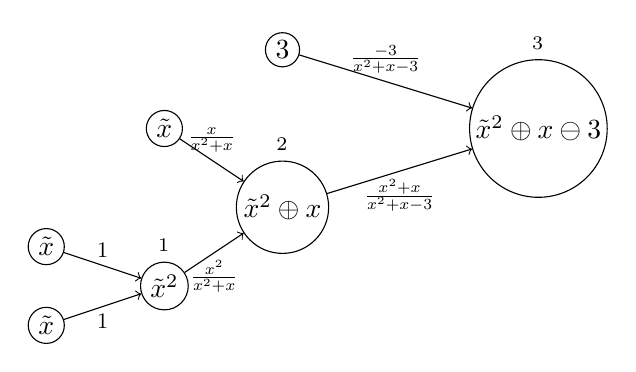
\begin{tikzpicture}
        [
            scale=.5,auto=left,
            important/.style={circle, draw=black, inner sep=1.5pt, minimum size=12pt},
            arrow/.style={-{Stealth[]}}
        ]
        \node[important] 
              (n1) at (1,0)  {$\tilde x$};
        \node[important] 
              (n2) at (1,2)  {$\tilde x$};
        \node[important, label={$\eps_1$}] 
              (n3) at (4,1)  {$\tilde x^2$};
        \node[important] 
              (n4) at (4,5)  {$\tilde x$};
        \node[important, label={$\eps_2$}] 
              (n5) at (7,3)  {$\tilde x^2 \oplus x$};
        \node[important] 
              (n6) at (7,7)  {$3$};
        \node[important, label={$\eps_3$}] 
              (n7) at (13.5,5) {$\tilde x^2 \oplus x \ominus 3$};
      
        \foreach \from/\to/\coeff in {n1/n3/{$1$},n3/n5/{$\frac{x^2}{x^2+x}$},n5/n7/{$\frac{x^2+x}{x^2+x-3}$}}
            \draw [->] (\from) to node[below, scale=0.8] {\coeff} (\to);
        
        \foreach \from/\to/\coeff in {n2/n3/{$1$},n4/n5/{$\frac{x}{x^2 + x}$},n6/n7/{$\frac{-3}{x^2 + x - 3}$}}
            \draw [->] (\from) to node[above, scale=0.8] {\coeff} (\to);
         
    \end{tikzpicture}
    \end{center}

    Il grafo è costruito nel seguente modo:
    \begin{itemize}
        \item si considera la sequenza di operazioni da svolgere: in questo caso \begin{enumerate}
            \item $z_1 \deq \tilde x \otimes \tilde x$
            \item $z_2 \deq z_1 \oplus \tilde x$
            \item $z_3 \deq z_2 \ominus 3 = g(\tilde x)$   
        \end{enumerate}
        \item si disegnano i nodi iniziali, ovvero quelli della prima operazione da svolgere, e sopra di essi si mettono gli errori commessi nel rappresentarli: siccome siamo interessati all'errore algoritmico partiamo già con numeri di macchina, quindi l'errore di rappresentazione è $0$ e lo omettiamo;
        \item si crea un nodo corrispondente a $z_1$: l'errore commesso nella creazione di questo nodo è l'errore locale del prodotto (qui chiamato $\eps_1$); 
        \item sopra gli archi che portano i nodi $\tilde x$ in $z_1$ indichiamo il coefficiente di amplificazione $c_x$ dei vari nodi: in questo caso sono entrambi uguali a $1$ poiché l'operazione è un prodotto;
        \item ripetiamo il procedimento: creiamo un nuovo nodo con $\tilde x$ e "errore di creazione" uguale a $0$ e lo usiamo per fare l'operazione di somma, creando un nuovo nodo (che corrisponde a $z_2$) con errore di creazione uguale all'errore locale della somma $\eps_2$;
        \item per ricavare i coefficienti di amplificazione sfruttiamo le formule ricavate prima, che ci dicono che nella somma $\tilde x^2 \oplus \tilde x$ i coefficienti di amplificazione sono dati da \[
            c_{x^2} = \frac{x^2}{x^2+x}, \qquad c_x = \frac{x}{x^2+x};
        \]
        \item ripetiamo un'ultima volta il ragionamento per quanto riguarda l'ultima operazione.
    \end{itemize}

    Possiamo ora calcolare l'errore totale a partire dal grafo: si parte dalla fine del grafo (nodo più a destra) e si calcola la somma tra l'errore del nodo (in questo caso $\eps_3$) e gli errori dei sottoalberi (calcolati ricorsivamente), moltiplicati per il loro coefficiente di amplificazione.

    Otteniamo quindi \begin{align*}
        \epsalg &= \eps_3 + \frac{x^2 + x}{x^2+x-3}(\dots) + \frac{-3}{x^2+x-3}\cdot 0\\
        &= \eps_3 + \frac{x^2 + x}{x^2+x-3}\parens*{\eps_2 + \frac{x^2}{x^2+x}(\dots) + \frac{x}{x^2+x}\cdot 0}\\
        &= \eps_3 + \frac{x^2 + x}{x^2+x-3} \parens*{\eps_2 + \frac{x^2}{x^2+x}(\eps_1 + 1\cdot 0 + 1 \cdot 0)}\\
        &= \eps_3 + \frac{x^2 + x}{x^2+x-3} \parens*{\eps_2 + \frac{x^2}{x^2+x} \cdot \eps_1}.
    \end{align*}
\end{example}

\subsection{Errore totale}

\begin{definition}
    [Errore totale]
        Si dice \strong{errore totale} del problema la quantità \[
            \epstot \deq \frac{g\parens[\big]{\tilde x} - f(x)}{f(x)}.
        \]
\end{definition}

Osserviamo chel'errore totale combina i concetti di errore inerente e algoritmico e ci dice quanto è grande l'errore nel calcolare $g$ con il valore di $\tilde x$ rispetto al calcolo esatto di $f(x)$.


Nell'\autoref{exmpl:func_error} abbiamo notato come l'errore totale fosse dato dalla somma dell'errore algoritmico e dell'errore inerente: questa relazione vale sempre, come dimostrato dal prossimo teorema.

\begin{theorem}
    \label{th:relation_eps_tot/alg/in}
    $\epstot \doteq \epsin + \epsalg$.
\end{theorem}
\begin{proof}
    In effetti si ha \begin{align*}
        \epstot &= \frac{g(\tilde x) - f(x)}{f(x)}\\
        &= \frac{g(\tilde x) - f(\tilde x) + f(\tilde x) - f(x)}{f(x)} \\ % 
        &= \frac{g(\tilde x) - f(\tilde x)}{f(x)} + \frac{f(\tilde x) - f(x)}{f(x)}\\
        &= \frac{g(\tilde x) - f(\tilde x)}{f(\tilde x)}\frac{f(\tilde x)}{f(x)} + \frac{f(\tilde x) - f(x)}{f(x)}\\
        &= \epsalg \cdot \frac{f(\tilde x)}{f(x)} + \epsin\\
        &= \epsalg \cdot \frac{f(\tilde x) - f(x) + f(x)}{f(x)} + \epsin\\
        &= \epsalg \cdot \parens*{ \frac{f(\tilde x) - f(x)}{f(x)} + \frac{f(x)}{f(x)} } + \epsin\\
        &= \epsalg \cdot (\epsin + 1) + \epsin\\
        &\doteq \epsalg + \epsin. \qedhere
    \end{align*}
\end{proof}

